%%%%%%%%%%%%%%%%%%%%%%%%%%%%%%%%%%%%%%%%%
% University Assignment Title Page 
% LaTeX Template
% Version 1.0 (27/12/12)
%
% This template has been downloaded from:
% http://www.LaTeXTemplates.com
%
% Original author:
% WikiBooks (http://en.wikibooks.org/wiki/LaTeX/Title_Creation)
%
% License:
% CC BY-NC-SA 3.0 (http://creativecommons.org/licenses/by-nc-sa/3.0/)
% 
% Instructions for using this template:
% This title page is capable of being compiled as is. This is not useful for 
% including it in another document. To do this, you have two options: 
%
% 1) Copy/paste everything between \begin{document} and \end{document} 
% starting at \begin{titlepage} and paste this into another LaTeX file where you 
% want your title page.
% OR
% 2) Remove everything outside the \begin{titlepage} and \end{titlepage} and 
% move this file to the same directory as the LaTeX file you wish to add it to. 
% Then add \input{./title_page_1.tex} to your LaTeX file where you want your
% title page.
%
%%%%%%%%%%%%%%%%%%%%%%%%%%%%%%%%%%%%%%%%%
%\title{Title page with logo}
%----------------------------------------------------------------------------------------
%	PACKAGES AND OTHER DOCUMENT CONFIGURATIONS
%----------------------------------------------------------------------------------------

\documentclass[11pt]{article}
\usepackage{comment}
\usepackage[english]{babel}
\usepackage{wrapfig}
\usepackage[utf8x]{inputenc}
\usepackage{amssymb,amsmath,amsthm}
\usepackage{graphicx}
\usepackage[colorinlistoftodos]{todonotes}
\usepackage{enumitem}
\usepackage{wrapfig}
\usepackage{listings}
\usepackage[font=tiny,labelfont=bf]{caption}
\usepackage{filecontents}
\usepackage{verbatim}
\usepackage{mathtools}
\usepackage{eurosym}
\usepackage{float}
\usepackage[numbers]{natbib}
\bibliographystyle{plainnat}
\setcitestyle{authoryear,open={(},close={)}}
\usepackage[export]{adjustbox}
\setlength\parindent{0pt}
\usepackage{parskip}
\usepackage{tikz}
\def\checkmark{\tikz\fill[scale=0.4](0,.35) -- (.25,0) -- (1,.7) -- (.25,.15) -- cycle;} 
\usepackage{hyperref}
\hypersetup{
    colorlinks,
    citecolor=blue,
    filecolor=black,
    linkcolor=black,
    urlcolor=blue
}
\usepackage[a4paper, total={6in, 8in}]{geometry}
\renewcommand{\thefigure}{\thesection-\arabic{figure}}
\tolerance=1
\emergencystretch=\maxdimen
\hyphenpenalty=10000
\hbadness=10000
\newcommand{\Lim}[1]{\raisebox{0.5ex}{\scalebox{0.8}{$\displaystyle \lim_{#1}\;$}}}


\begin{document}
\begin{titlepage}

\newcommand{\HRule}{\rule{\linewidth}{0.7mm}} % Defines a new command for the horizontal lines, change thickness here

\center % Center everything on the page
 
%----------------------------------------------------------------------------------------
%	HEADING SECTIONS
%----------------------------------------------------------------------------------------

\textsc{\LARGE Leiden University}\\[1cm] % Name of your university/college
\textsc{\Large An AMUSE Based Research Project}\\[0.5cm] % Major heading such as course name
%\textsc{\large Assignment 1}\\[0.5cm] % Minor heading such as course title

%----------------------------------------------------------------------------------------
%	TITLE SECTION
%----------------------------------------------------------------------------------------

\HRule \\[0.5cm]
{ \LARGE \textbf{\uppercase{ The Milky Way and its exotic Millisecond Pulsar Population: \\ A Statistical Analysis}}\\[0.29cm]
\small \textit{Is there the possibility that a non-negligible fraction of millisecond pulsars living in the Milky Way migrated from the Large Magellanic Cloud?}}\\[0.29cm] % Title of your document
\HRule \\[1cm]
 
%----------------------------------------------------------------------------------------
%	AUTHOR SECTION
%----------------------------------------------------------------------------------------

\begin{minipage}{0.4\textwidth}
\begin{flushleft} \large
\emph{Author:}\\
Shiyang \textsc{ Zhang} \textit{(s2746425)}\\ Arend \textsc{ Moerman} \textit{(s1749323)}\\ Erwan\textsc{ Hochart} \textit{(s2009296)} \\
\end{flushleft}
\end{minipage}
~
\begin{minipage}{0.5\textwidth}
\begin{flushright} \large
\emph{Supervisor:} \\
Prof.dr. Simon \textsc{Portegies Zwart} \\
Martijn \textsc{Wilhelm}\\
\end{flushright}
\end{minipage}\\[1cm]

% If you don't want a supervisor, uncomment the two lines below and remove the section above
%\Large \emph{Author:}\\
%John \textsc{Smith}\\[3cm] % Your name

%----------------------------------------------------------------------------------------
%	DATE SECTION
%----------------------------------------------------------------------------------------

{\large \today}\\[2cm] % Date, change the \today to a set date if you want to be precise

%----------------------------------------------------------------------------------------
%	LOGO SECTION
%----------------------------------------------------------------------------------------


\includegraphics[width=300px, keepaspectratio]{logo-univ-leidenobservatory-transparent.png}\\[1cm] % Include a department/university logo - this will require the graphicx package
 
%----------------------------------------------------------------------------------------

\vfill % Fill the rest of the page with whitespace
\pagenumbering{gobble}
\end{titlepage}

\section*{Abstract}


\newpage
\tableofcontents



\newpage
\pagenumbering{arabic}
\section{Introduction}\label{Introduction}
\setcounter{figure}{0} 
From being used to detect the first extra-solar planetary system \citep{Planet} to being the centre of discussion in Nobel Prize-winning papers testing the theory of general relativity \citep{NobelPrize}, millisecond pulsars have become a popular research topic in the field of physics since their discovery in 1967 \citep{Bell}.

Pulsars are rapidly rotating neutron stars formed after a supernova explosion which periodically emits electromagnetic radiation as charged particles accelerate along their magnetic field lines. This periodic and stable emission of signals is the source behind their broad use within the field. To date, there are upwards of 2800 detected pulsars \citep{AustraliaPulsar} and figure \ref{PulsarPopMap} shows the distribution of their population within the Milky Way.

\begin{figure}[htbp]
\centering
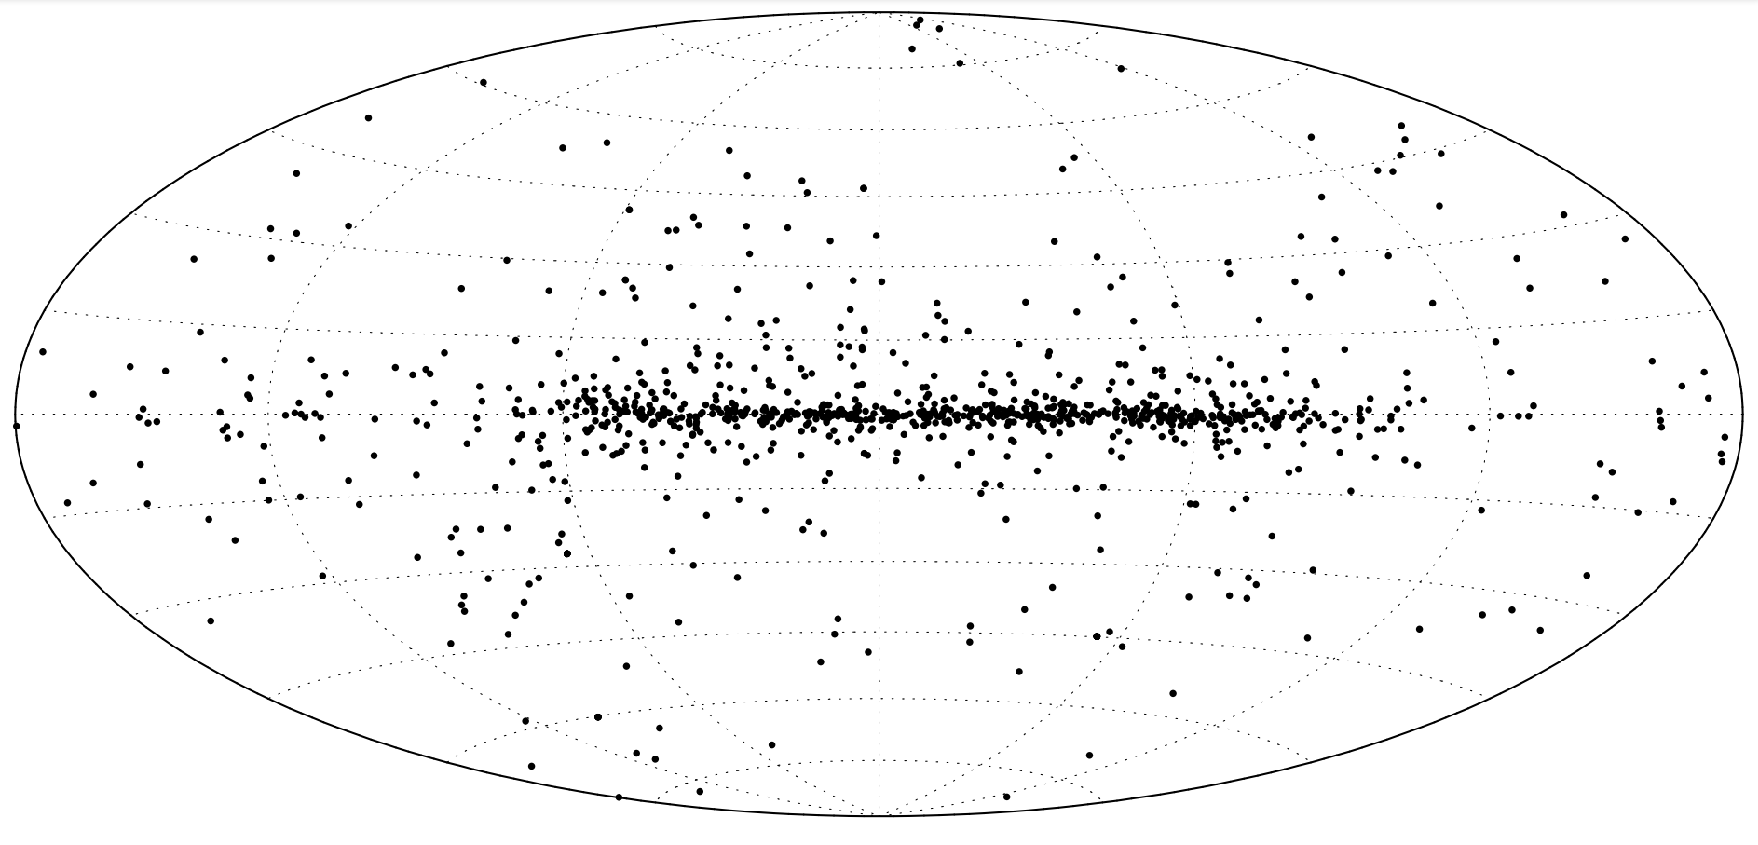
\includegraphics[scale=0.45]{Pulsars.pdf}
\caption{The population map of pulsars within the Milky Way. The plane of the galaxy can be denoted with the horizontal line of the pulsar population. (image courtesy of \cite{Lorimer2001})}
\label{PulsarPopMap}
\end{figure}

Although there has been a vast amount of research conducted regarding pulsars, there is still an abundance of questions left unanswered. One such mystery is the significant fraction of millisecond pulsars within the Milky Way having no companions. Although it's proposed that these millisecond pulsars may have gotten rid of their companions via ablation, which seems to be the case for PSR 1957 +20 \citep{Ablation}, the timescales of such a process make this explanation inconclusive. One possible reason for this observed fraction of solitary pulsars that have yet to be touched upon by research may be the capturing of millisecond pulsars from nearby galactic systems such as the Large Magellanic Cloud (hereafter LMC) or Small Magellanic Cloud (hereafter SMC). This paper takes a statistical approach with the help of AMUSE$^{[1]}$ \citep{AMUSE} in investigating the possibility of millisecond pulsars migrating from the LMC to the Milky Way.

\vfill
{\tiny [1] Code available at: https://amusecode.github.io/}

\subsection{Outline of the paper}

The paper is composed of six main sections. Section two gives a brief introduction of millisecond pulsars providing the reader with justification as to why such a topic is interesting to investigate. Section three dissects the mathematical theory implemented within our code, giving for a better understanding of the eventual results. An overall discussion on AMUSE and the code is found in section four in which we also justify some further assumptions made. Section five and six describes the general procedure and discusses the results of the paper respectively. Section seven will summarise the report with a general conclusion as well as suggesting possible research that can be built from our paper.


\section{Millisecond Pulsars: What are they?}

The millisecond pulsar birthrate in the Milky Way is $2\times10^{-5}$ yr$^{-1}$ \citep{Lorimer1999} and forms once a massive star loses its fuel, causing it to no longer sustain hydrostatic equilibrium and collapse onto itself. If the star is massive enough, it will cause a supernova explosion in which the remaining object, the neutron star, ends up weighing around $1.4M_\odot$ with a significant portion of the original mass ejected from the system. Since the star is now only a fraction of its original size (a few kilometres in radius), for it to conserve angular momentum, it's spin drastically increases. The periodic signal received from these celestial objects stems from the fact that charged particles accelerate along the magnetic field lines and as the pulsar rotates along its axis if the beam passes our line of sight a signal is detected. It is noteworthy to mention, however, that it is still unclear how their magnetic field arises \citep{Magnetic} but this is out of the scope of the paper.

This report focuses on a particular class of pulsars called millisecond pulsars. These pulsars have a period $T$ of $1.4 \leq T$ ms $\leq 30$ \citep{Lorimer2008}, meaning they can spin just shy of a thousand times per second along their axis. The report investigates this class of pulsar specifically as a quicker spin induces a weaker magnetic field, in turn, allowing them to live longer \citep{Phinney}. A `normal' pulsar tends to live around $100$ Myr \citep{Toscano}, whereas, millisecond pulsars have a lifetime comparable to the age of the Universe \citep{Lorimer2008}, allowing the opportunity to be captured within the Milky Way without us even realising they may have originated from another system.

However, a typical supernova explosion will not yield the rapid spin millisecond pulsars exhibit. To obtain its rotational speed millisecond pulsars need to originate from a binary system.  In this binary system, the massive star dies first and goes through a supernova explosion following the same procedure described earlier. If the binary system remains bounded, the resulting neutron star may start to accrete mass from its companion causing its angular momentum (and therefore spin) to increase \citep{NRAO}. Due to the globular cluster being the densest region of the galaxy, they are somewhat of a nursery for millisecond pulsars since there is a larger probability for a neutron star to interact with another celestial object to increase their spin in these regions. 

As the millisecond pulsar accretes mass, the orbit of the system starts to contract emitting gravitational potential energy and giving rise to the possibility for the system to become unbound \citep{Kulkarni1995}. Another possible scenario for the system to be disrupted is one in which a second supernova explosion, this time of the companion star, occurs, causing the millisecond pulsar to get ejected. Nevertheless, these two scenarios are not the norm with $80\%$ of detected millisecond pulsars being found in binary systems \citep{Lorimer2008}.


\section{Distribution of our Millisecond Pulsars}\label{MathematicalTheory}
\setcounter{figure}{0} 

\subsection*{The Velocity Distribution}\label{Velocity}
As alluded to in the previous section, millisecond pulsars tend to live in binary systems. Pulsars in a binary system have low velocities and therefore will never get unbound from the LMC. For this reason, one assumption we make is that all millisecond pulsars in our simulation get ejected via a secondary supernova explosion initiated by their companions. We apply this assumption by changing the time interval in which millisecond pulsars are born at (further discussed in section \ref{TheSimulation}). 

Although a supernova explosion can be symmetric in the dying stars frame, this is not the case in the centre-of-mass frame. The millisecond pulsar will feel a rebound effect after its partner's supernova explosion and in turn, get a boost in its velocity. If half the systems mass gets ejected during the supernova event the binary system is destroyed \citep{Hills} and the millisecond pulsar may obtain a velocity high enough to become unbound from the LMC.

There have been many papers investigating the velocity distribution of pulsars over the past few decades (\cite{Lorimer} ; \cite{Hansen1997} ; \cite{Toscano1999} ; \cite{Hobbs2005}) each providing differences in their results. This paper uses \cite{Hansen1997} as a reference point simply due to it calculating the ejection velocities for pulsars after a supernova ejection which is the scenario that allows the pulsars to become unbound from the LMC. Furthermore, this velocity distribution is used since it takes into account the fainter, quicker pulsars as well as the slower, brighter ones that some of the other studies overlooked. Using Monte Carlo simulations, they found that pulsars ejected from a supernova tend towards the following velocity distribution:

\begin{equation}
    P(v_k) = \sqrt{\frac{2}{\pi}}\frac{\bar{v}^2}{\sigma^3_v}e^{-v_k^2/2\sigma_v^2}
\end{equation}

Where $\bar{v}$ is the mean velocity of the population, $\sigma_v$ the standard deviation of the distribution and $v_k$ the kick velocity. Upon simulation, they found that the mean velocity is given as $\bar{v}_k = 250-300$ km s$^{-1}$ with a standard deviation of $\sigma_v = 190$ km s$^{-1}$. The mean velocity for this paper was chosen at $\bar{v_k} = 250$ km s$^{-1}$ while keeping the standard deviation at $\sigma_v = 190$ km s$^{-1}$. The distribution function of equation 1 with the chosen values for this paper is shown in figure \ref{CDFPDF}.

\begin{figure}[H]
\centering
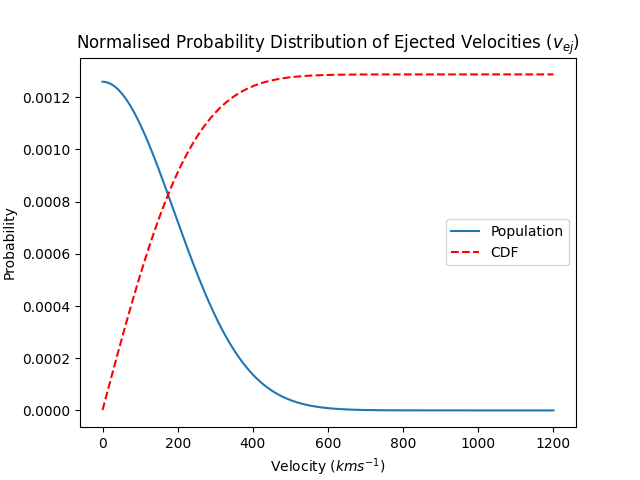
\includegraphics[scale=0.46]{CDFPDFVelocities.png}
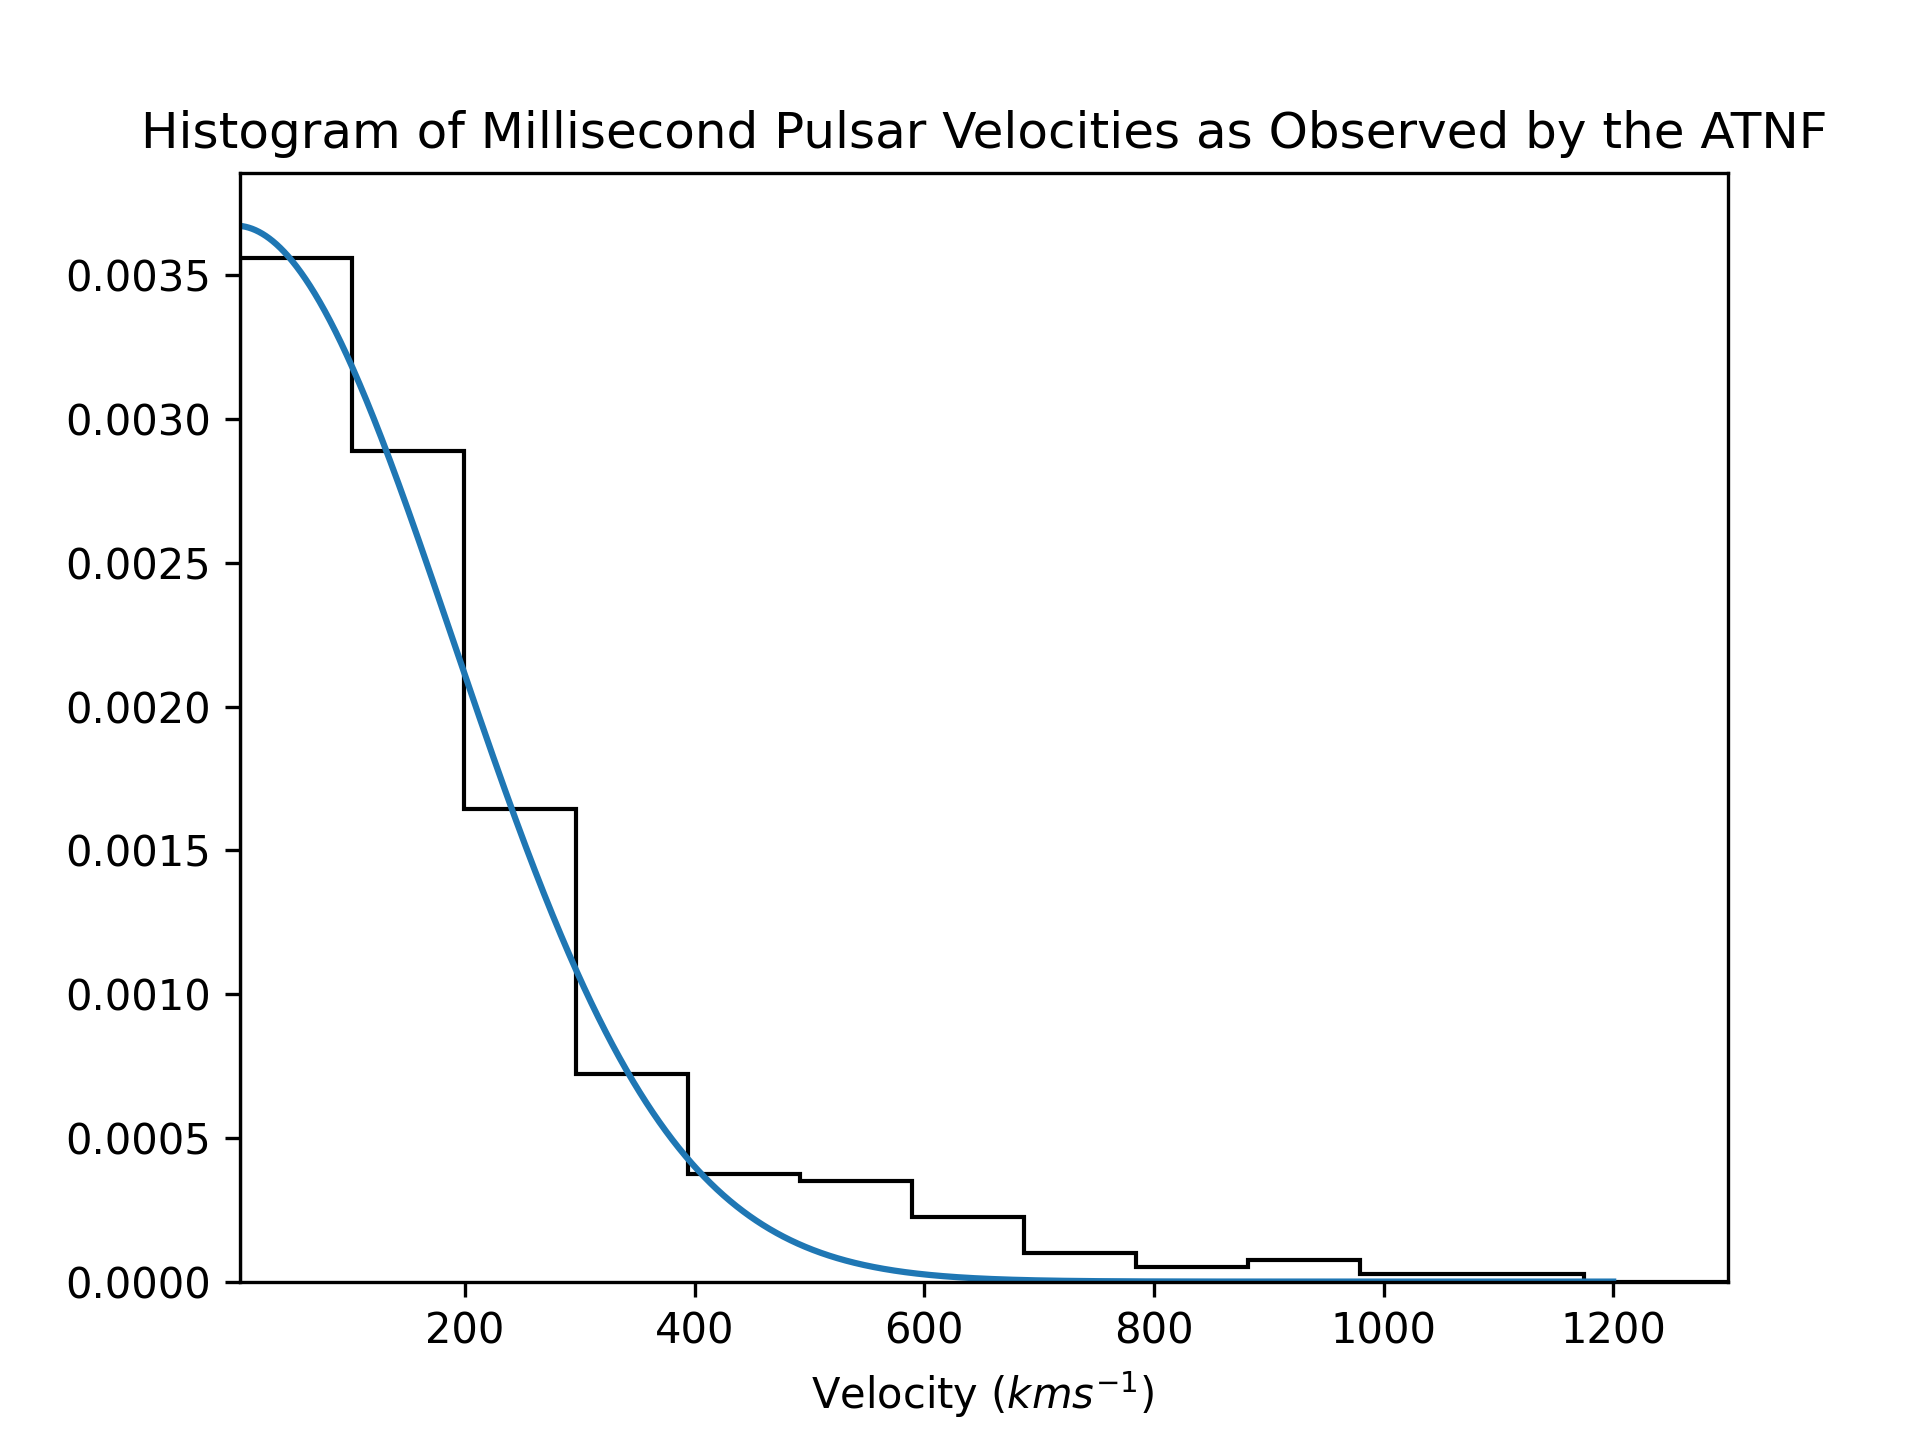
\includegraphics[scale=0.46]{Histogram.png}
\caption{Left: Normalised distribution function and cumulative distribution function (CDF) of the velocities in our simulation. Right: Histogram of pulsar velocities in km s$^{-1}$ using the ATNF catalogue \citep{AustraliaPulsar}}
\label{CDFPDF}
\end{figure}

As can be seen in the figure above, most millisecond pulsars will have their velocities in the lower end of the spectrum. This trend fits that of the observed data with the histogram shown on the right-hand side, further showing the strength of the chosen velocity distribution of the report. To improve the ejection mechanism the code randomly multiplies the $v_x, v_y, v_z$ values by $-1$ or $1$ such that the direction of ejection is random.

\subsection{The Mass Distribution}

Another aspect to keep in mind with the simulated millisecond pulsars is the mass attributed to them. Although this will not play a role in the orbit and evolution of the system, it is defined as it allows calculation on the energy of the system. Calculating the energy of the system provides information on the reliability and stability of the simulation.

Although pulsars tend to have a mass of $1.4M_\odot$ following the Chandrasekhar limit, millisecond pulsars accrete mass after their supernova explosion meaning they can attain a mass exceeding this. The mass distribution for the sampled population adopted in this report uses a Gaussian distribution utilising the values found by \cite{Antoniadis2016} as this is one of the more recent works investigating the issue. The Gaussian distribution is taken simply due to the lack of papers providing a mass distribution towards the population. Furthermore, the Central Limit Theorem states that distributions tend to a normal distribution at a large enough sample size limit. \cite{Antoniadis2016} found that at least $3\%$ of all millisecond pulsars have a mass above $2.1 M_\odot$ which allowed the calculation of the standard deviation when working backwards. Furthermore, the paper constrains the maximum mass as $2.15 M_\odot$ while stating that the average mass of the millisecond pulsar population being between $1.3 \leq \bar{M}_\odot \leq 1.5$.



\section{The Code}\label{TheoryBehindtheCode}
\setcounter{figure}{0} 

The code is built around three main parts; the gravitational potentials used, the millisecond pulsar formation rate and the tracking of the orbit.

\subsection{Gravitational Potentials}

The simulation incorporates four gravitational potentials, one for the SMC, one for the LMC, one for the globular cluster the millisecond pulsar is shot out from and finally, one for the Milky Way. The potentials are based on code imported from the AMUSE community \texttt{galactic\_potentials}.

The potential of the LMC and SMC incorporates both a Plummer and Navarro–Frenk–White (NFW) potential \citep{Navarro1997}. Although this gives for an idealised version of the potential for these two irregular galaxies, numerous papers have approximated their potentials as such with great success (\cite{Besla}; \cite{Yoshizawa}; \cite{Bekki}). The SMC, being the smallest galactic system, will have minimal effect on the trajectory of the pulsar and a general model of its potential suffices for the report. Furthermore, although the pulsar originates from the LMC, given that it has to be ejected from the system to be captured by the Milky Way the pulsar's trajectory will be minimally affected by the LMC potential meaning that it is right to ignore some of the finer details. Lastly, the paper isn't interested in the intricate details of the evolution of the pulsar within these systems instead it aims to find which parameters are needed for the pulsar to be bound to the Milky Way.

The Milky Way potential is taken from the one developed by \cite{Bovy2015}, namely \texttt{MWpotentialBovy2015}. This code also provides an idealised version of the potential however it incorporates a bulge model with a power-law density profile along with a Miyamoto-Nagai potential describing the disk and an NFW potential for the dark matter halo. His paper provides extensive details if one wishes to know further. However, it is noteworthy to realise that both the spiral arms and bar of the Milky Way are ignored in this profile, nevertheless, it provides an accurate representation of the general galactic potential.

The globular cluster will have the weakest potential within the simulation. However, since the millisecond pulsar originates at this location, it is essential to represent such a system. The globular cluster mimics the cluster NGC 1783 which inhabits the LMC. The potential used will be that of a Plummer potential as this profile was first introduced to imitate globular cluster environments \citep{Plummer}.

One final comment on the potentials is that they are rigid potentials, this means that neither the LMC, SMC, globular cluster or Milky Way are evolving throughout the simulation and therefore will have no interaction with one another including tidal effects. Although this is a large assumption, as mentioned earlier, the report doesn't look to analyse in intricate detail the trajectory of the millisecond pulsar, instead, it looks at whether the millisecond pulsar ends up being bound to the Milky Way and therefore potentials which interact would only add unnecessary complication to the code and yield it inefficient.

\subsection{Supernova Timing}

\subsection{Bridging Systems}\label{Bridge}

\subsection{Tracking the Orbit}

\section{The Simulation}\label{TheSimulation}
\setcounter{figure}{0} 

The simulation begins by initialising the LMC, SMC and Milky Way system. The SMC and LMC's position and velocity parameters are provided by SIMBAD \citep{Simbad} and can be referenced in table \ref{TableLMCSMC} and table \ref{velvalues}. The heliocentric frame which the data is based on gets converted into the galactocentric frame with the help of \texttt{astropy}. This conversion enables the Milky Way to become the frame of reference. After evolving the system backwards 1Gyr in time, the globular cluster, modelled after the LMC's NGC 1783, is added to the system whose initial values are also shown in table \ref{velvalues}. The code traces the system backwards by reversing the velocity's sign in the gravitational code. The research then initialises the system at this time and takes the values found as the new initial conditions. By doing so we do not take into account the stellar formation rate history nor the evolution of the different potentials and so our initial values may differ to what the actual scenario was $1$Gyr back in time.

\begin{table}[htb]
\begin{center}
\begin{tabular}{lcccccccc}
\hline
Object & R.A (ICRS system) & Dec. (ICRS system) & Distance (kpc)  \\ \hline
LMC &  05h 23m 34.6s    &    $-69^{\circ} 45' 22''$      & 49.97   \\
SMC&	00h 52m 38.0s   &    $-72^{\circ} 48' 01''$  & 61.7  \\
Globular Cluster &   04h 59m 08.6s    &    $-65^{\circ} 59' 15''$  & 50.1 \\ \hline
\end{tabular}
\caption{Initial (heliocentric) positional values of the LMC, SMC and NGC 1783 used for the simulation. Data was taken from \cite{Simbad}, except for the distance of NGC 1783, taken from}
\label{TableLMCSMC}
\end{center}
\end{table}

\begin{table}[htb]
\begin{center}
\begin{tabular}{lcccccccc}
\hline
Object & $v_x$ (km s$^{-1}$) & $v_y$ (km s$^{-1}$) & $v_z$ (km s$^{-1}$)  \\ \hline
LMC &  47.0 & 242 & 225   \\
SMC&	5.35 & 164 & 136 \\\hline
\end{tabular}
\caption{Initial (heliocentric) velocity values of the LMC and SMC. Data was taken from \cite{Simbad}. The velocity of the globular cluster is calculated from the circular velocity formula at a given radius due to the minimal amount of measurements regarding the velocity of NGC 1783.}
\label{velvalues}
\end{center}
\end{table}

\newpage

The globular cluster is assumed to be a collisionless system such that the millisecond pulsar doesn't have it's trajectory drastically alter at the beginning of each ejection. A collisionless cluster was chosen for the paper as it reduces the dependency on arbitrary parameters such as the number of particles within the globular cluster or the proximity they have with one another. Furthermore, for large velocities, neighbouring stars will have a negligible effect on an unbound pulsar.

The simulation then proceeds by evolving the system forwards in time for 1Gyr with the help of the bridge code mentioned in section \ref{Bridge}, allowing for the multi-scale system to be represented at the current time with the emitted millisecond pulsars having their final positions being their positions now. By moving forwards in time, once again we neglect the stellar formation rate of all three galactic systems which may play a role in the overall mass and therefore the potential of the system. Nevertheless, we assume that the LMC emits an isolated millisecond pulsar from a supernova every $1.80$ Myr. 

This emission rate of one millisecond pulsar every $1.80$ Myr is based on the average star formation rate (SFR) of both the Milky Way and LMC in the last $2$Gyr, found to be  $0.68-1.45$ $M_\odot$ yr$^{-1}$ \citep{Thomas} and $0.2 M_\odot$ yr$^{-1}$ \citep{Harris} respectively. Using the fact that millisecond pulsars are born every $5\times10^4$ years in the Milky Way \citep{Lorimer2008}, the ratio of the SFR between both systems was taken to obtain the final birth rate of millisecond pulsars within the LMC. Using this information a millisecond pulsar is born every $0.36$ Myr in the LMC when using an SFR of $1.45 M_\odot$ for the Milky Way. Given the fact that $20\%$ of all millisecond pulsars are in non-binary systems \cite{Lorimer2008} and the report only looks at non-binary millisecond pulsars, this gives for a final value of a millisecond pulsar birth occurring every $1.80$ Myr in the LMC.

It is clear from this that many assumptions are made - for instance taking a $1:1$ relation between the birth rate of millisecond pulsars in the LMC and Milky Way as well as the arbitrary value used for the SFR of the Milky Way. However, given the information currently provided this can be deemed as a sufficiently accurate representation of the non-binary millisecond pulsar population of the LMC.

In the end, a total of $555$ millisecond pulsars get simulated, and so given the velocity distribution, it is expected that only a minute fraction of these gets captured by the Milky Way. To further simplify data processing, the code filters through the data by only extracting the bound pulsars, defined as millisecond pulsars within $\pm 20$kpc from the galactic centre in all three spatial coordinates $(x, y, z)$.



\newpage
\section{Results}\label{Results and Discussion}
\setcounter{figure}{0} 
\subsection{A Qualitative Analysis}\label{Qualitative}

\begin{figure}[H]
\centering
\includegraphics[width=.8\textwidth]{neutron_star_trajectories_xy_1.png}
\includegraphics[width=.49\textwidth]{neutron_star_trajectories_xz_1.png}
\includegraphics[width=.49\textwidth]{neutron_star_trajectories_yz_1.png}
\caption{Top: Captured millisecond pulsar trajectories in the $xy$ plane. The Milky Way is shown with the contour lines of its potential. Bottom Left: Captured millisecond pulsar trajectories in the $xz$ plane. Bottom right: Captured millisecond pulsar trajectories in the $yz$ plane.}
\label{PersistenceErwanComp}
\end{figure}


\subsection{A Quantitative Analysis}\label{Quantitative}

\subsection{Noise and Error}

Figure \ref{Energy} shows the ratio of the energy $E(t)$ at a given time $t$ with respect to the initial energy $E_0$ of the simulation. One observes from this figure that the energy varies drastically over the evolution of the system, plateauing as the time approaches $2$ Gigayears to a value of $XXXX$. This large periodic variation, signified by the thicker lines, suggests that the system is unstable in the beginning of the simulation and this instability stems from the many assumptions taken when modelling the galactic system. 

One of the assumptions in the report was that the potentials were rigid and will not interact with one another. This means that when systems are approaching one another, upon their closest encounter the large tidal forces felt will be energy unaccounted. This fact is highlighted in the figure since the trough of the graph, occurring at $XXXXX$ Myr, is the moment of closest approach between the LMC and the Milky Way. The fact that the energy ratio plateau's after this closest approach further signifies the uncertainties brought from assuming rigid potentials. Once the two galactic systems start to distance from one another, the tidal forces felt of either system decreases making the total energy of the system approach it's initial value. One can observe however that it doesn't converge back to $E/E_0 = 1$, rather it converges to $XXXX$ meaning there is only a $XXX\%$ loss of energy which is somewhat reasonable.

\section{Conclusion}\label{Conclusion}
\setcounter{figure}{0} 


\newpage
\bibliography{references}

\newpage
\section*{Appendix A: Graphs of the other simulations used}\label{AppA}
\counterwithin{figure}{section}
\renewcommand{\thefigure}{A.\arabic{figure}}
\setcounter{figure}{0}

\begin{figure}[H]
\centering
\includegraphics[width=.75\textwidth]{neutron_star_trajectories_xy_2.png}
\includegraphics[width=.75\textwidth]{neutron_star_trajectories_xz_2.png}
\includegraphics[width=.75\textwidth]{neutron_star_trajectories_yz_2.png}
\caption{Top: Captured millisecond pulsar trajectories in the $xy$ plane. The Milky Way is shown with the contour lines of its potential. Bottom Left: Captured millisecond pulsar trajectories in the $xz$ plane. Bottom right: Captured millisecond pulsar trajectories in the $yz$ plane.}
\label{Simulation2}
\end{figure}

\begin{figure}[H]
\centering
\includegraphics[width=.75\textwidth]{neutron_star_trajectories_xy_3.png}
\includegraphics[width=.75\textwidth]{neutron_star_trajectories_xz_3.png}
\includegraphics[width=.75\textwidth]{neutron_star_trajectories_yz_3.png}
\caption{Top: Captured millisecond pulsar trajectories in the $xy$ plane. The Milky Way is shown with the contour lines of its potential. Bottom Left: Captured millisecond pulsar trajectories in the $xz$ plane. Bottom right: Captured millisecond pulsar trajectories in the $yz$ plane.}
\label{Simulation3}
\end{figure}

\begin{figure}[H]
\centering
\includegraphics[width=.75\textwidth]{neutron_star_trajectories_xy_4.png}
\includegraphics[width=.75\textwidth]{neutron_star_trajectories_xz_4.png}
\includegraphics[width=.75\textwidth]{neutron_star_trajectories_yz_4.png}
\caption{Top: Captured millisecond pulsar trajectories in the $xy$ plane. The Milky Way is shown with the contour lines of its potential. Bottom Left: Captured millisecond pulsar trajectories in the $xz$ plane. Bottom right: Captured millisecond pulsar trajectories in the $yz$ plane.}
\label{Simulation4}
\end{figure}

\begin{figure}[H]
\centering
\includegraphics[width=.75\textwidth]{neutron_star_trajectories_xy_5.png}
\includegraphics[width=.75\textwidth]{neutron_star_trajectories_xz_5.png}
\includegraphics[width=.75\textwidth]{neutron_star_trajectories_yz_5.png}
\caption{Top: Captured millisecond pulsar trajectories in the $xy$ plane. The Milky Way is shown with the contour lines of its potential. Bottom Left: Captured millisecond pulsar trajectories in the $xz$ plane. Bottom right: Captured millisecond pulsar trajectories in the $yz$ plane.}
\label{Simulation5}
\end{figure}

\newpage
\section*{Appendix B: Graph showing all the millisecond pulsar trajectories}\label{AppA}
\counterwithin{figure}{section}
\renewcommand{\thefigure}{B.\arabic{figure}}
\setcounter{figure}{0}


\begin{figure}[H]
\centering
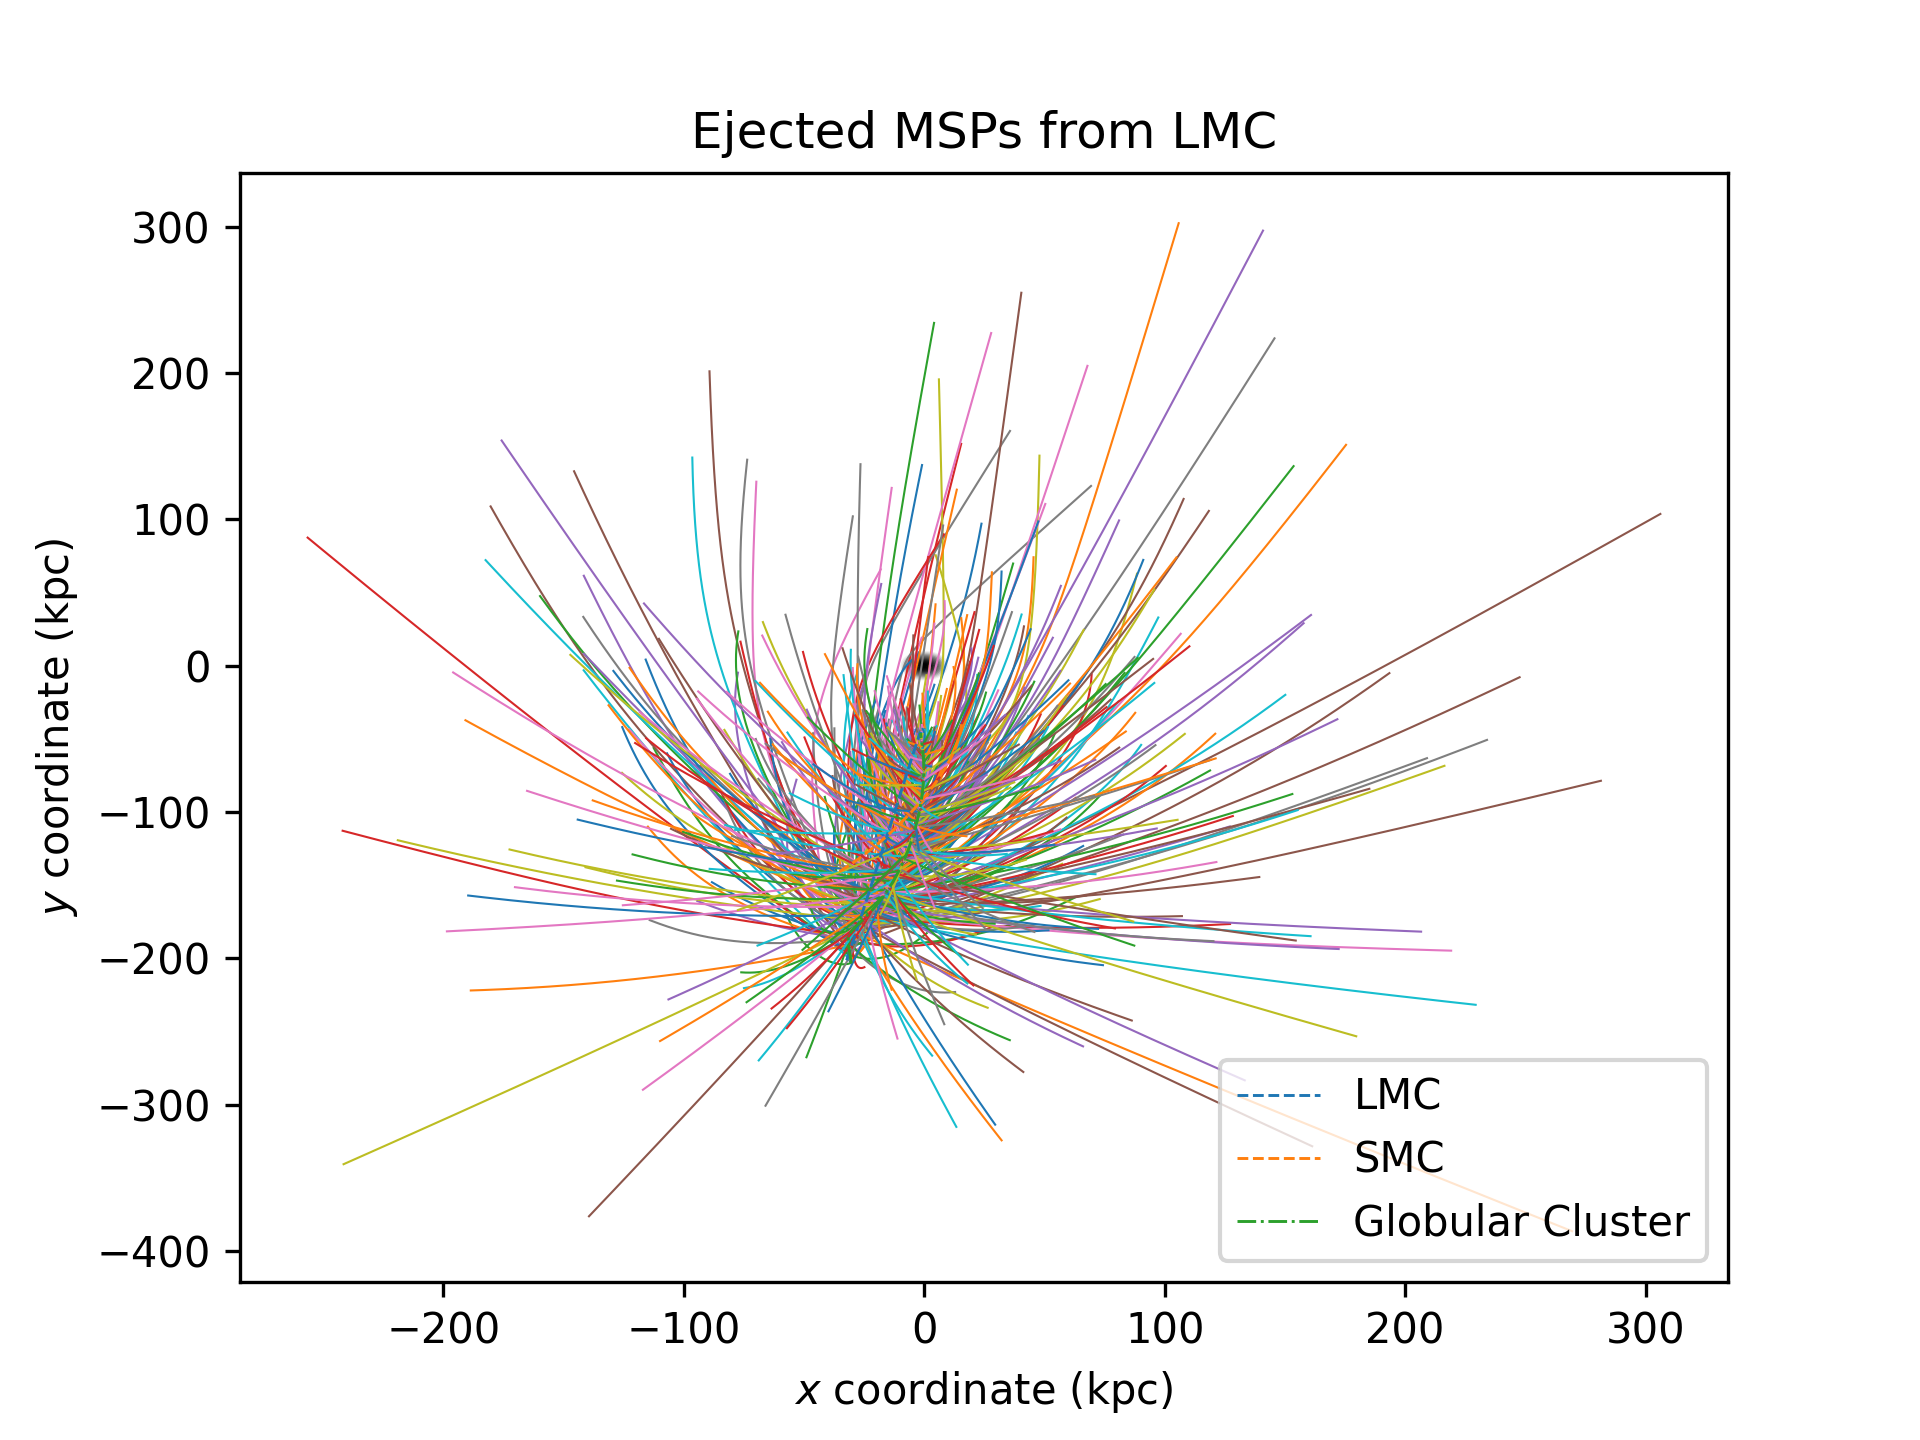
\includegraphics[width=1\textwidth]{AllNeutronStarsEmitted.png}
\caption{Graph showing all the emitted millisecond pulsars during one run of a simulation.}
\label{Simulation6}
\end{figure}

\end{document}